\subsection{ソフトウェアエンジニアリング運用計画}

運用計画は、ソフトウェアを運用し続けるための準備を体系化する活動である。運用は多くの場合、開発期間より長く続く。したがって、運用計画では、短期の配備だけでなく、長期の保守、支援、容量、サービス水準、コスト、人員、供給者、セキュリティを考える必要がある。

運用担当技術者は、作業手順やツールを、目的に合う形で文書化する。証拠として残すべきものには、方針と計画、サービス文書、手順、プロセス、プロセス制御記録がある。

\subsubsection{運用計画と供給者管理}

\paragraph{運用計画}

運用計画は、プロジェクト要求、開発者や保守担当者のニーズを、運用サービスへ翻訳する活動である。開発は数か月から数年で終わることが多いが、運用は何年も続く。そのため、資源見積もり、人員計画、教育、予算、容量、支援体制を早くから考えることが重要である。

新しいソフトウェアを開発すると決めた時点で、運用と保守の要求を考慮すべきである。概念文書、運用保守計画、運用構想（Concept of Operations, CONOPS）を作り、利用者が変更要求や問題報告をどのように出すか、誰が受け付けるか、どのように優先順位を付けるか、どのようにリリースへ反映するかを明らかにする。

\par\smallskip\noindent\refstepcounter{table}\label{tab:ch06-04}\textbf{表 \thetable: 第06章 ソフトウェアエンジニアリング運用 表04}\par\smallskip
\begin{longtable}{L{45mm}L{105mm}}
\toprule
運用計画で扱う項目 & 説明 \\
\midrule
役割と責任 & 新しいサービスまたは変更されたサービスを、誰が実装、運用、保守するかを決める。 \\
顧客と供給者の活動 & 顧客側と供給者側が行う作業、契約、合意を明確にする。 \\
要員と教育 & 必要な人員、技能、訓練、技術支援を計画する。 \\
プロセスとツール & 使う手順、測定、方法、ツールを定義する。 \\
容量と財務 & 将来の利用量、予算、時程、費用を見積もる。 \\
サービス受け入れ基準 & 運用開始できると判断する条件を決める。 \\
期待成果 & 運用した結果として何を測定し、どの水準を満たすかを数値で表す。 \\
\bottomrule
\end{longtable}

個々の問題報告や変更要求のレベルでは、対象となるリリース日、次版の内容、潜在的な衝突、リスク、ロールバック計画、データ移行計画、関係者への通知を扱う。

\begin{figure}[htbp]
\centering
\IfFileExists{assets/generated_figures/ch06/fig-ch06-03.png}{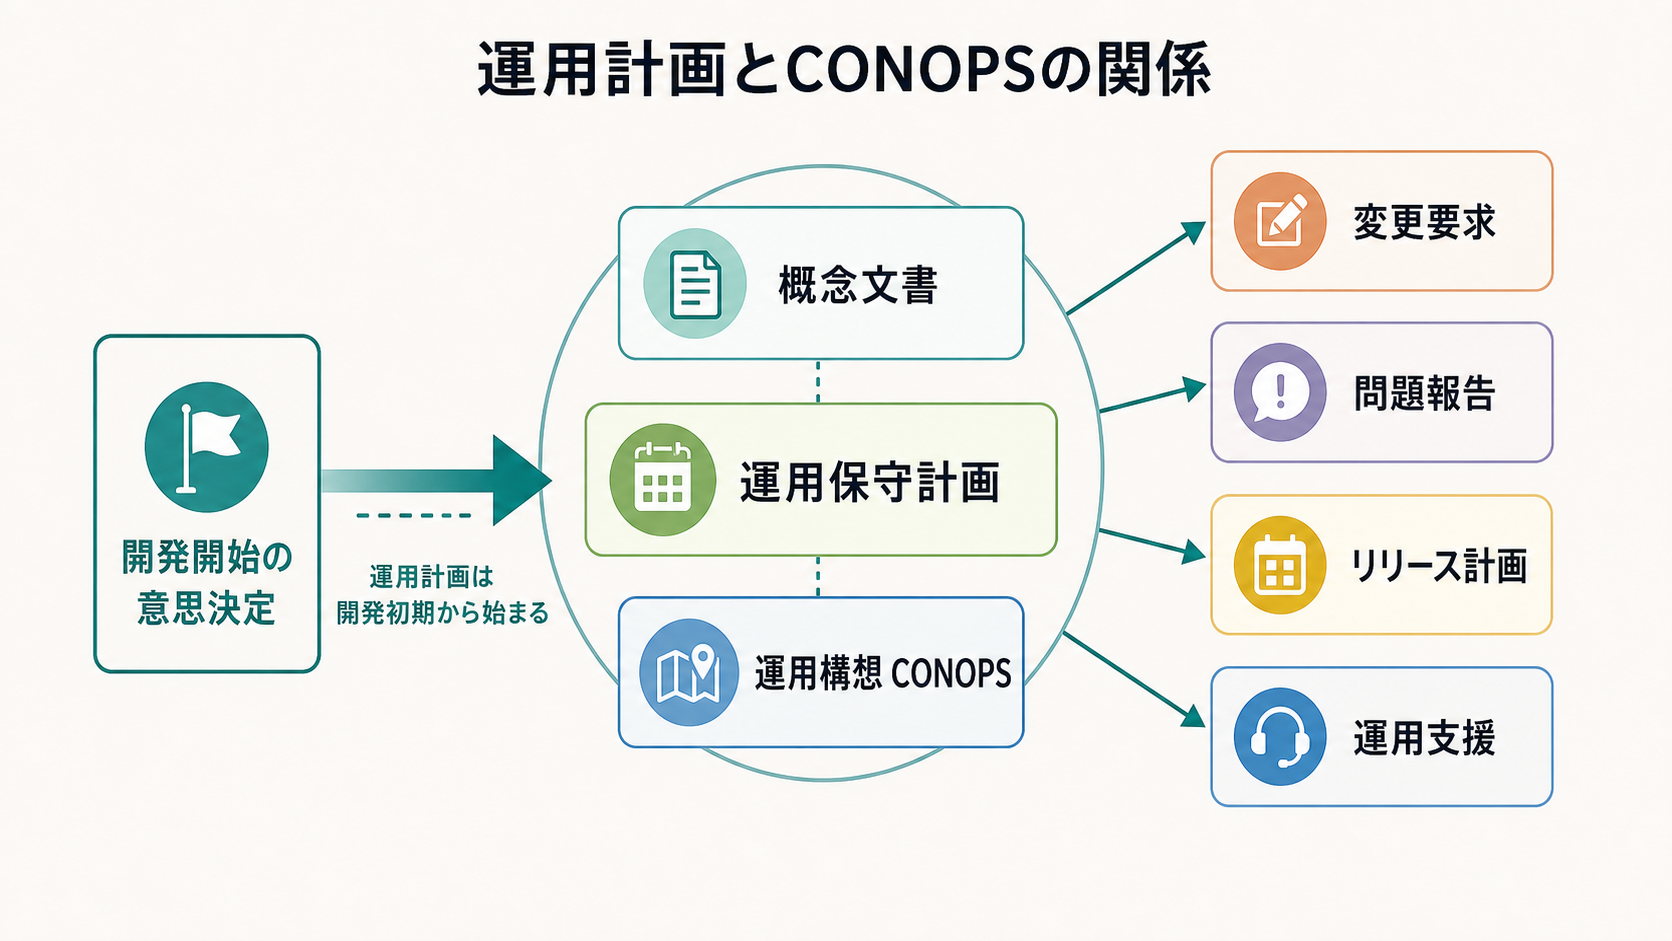
\includegraphics[width=0.96\linewidth]{assets/generated_figures/ch06/fig-ch06-03.png}}{\fbox{\parbox[c][48mm][c]{0.9\linewidth}{\centering 画像生成待ち\\運用計画とCONOPSの関係}}}
\caption{運用計画とCONOPSの関係}
\label{fig:ch06-03}
\end{figure}

\paragraph{供給者管理}

供給者管理とは、外部供給者の製品やサービスを、品質の高い運用サービスに結びつくように管理する活動である。ここでいう供給者には、外部委託先、クラウドサービス、インフラ提供者、プラットフォーム提供者、監視ツール提供者などが含まれる。

運用担当技術者は、供給者との関係を、製品やサービスの性質に合わせて決める。たとえば、サービスとしてのインフラ（IaaS）やサービスとしてのプラットフォーム（PaaS）を使う場合、契約、責任分界点、可用性、障害通知、データ保護、監査、終了時の移行を確認しなければならない。

\subsubsection{開発環境と運用環境}

ソフトウェアプロセスでは、開発環境、試験環境または品質保証環境、事前本番環境、本番環境が使われる。品質を作り込み、本番リリースのリスクを下げるには、これらの環境が一貫しており、本番環境と同期している必要がある。

\par\smallskip\noindent\refstepcounter{table}\label{tab:ch06-05}\textbf{表 \thetable: 第06章 ソフトウェアエンジニアリング運用 表05}\par\smallskip
\begin{longtable}{L{35mm}L{115mm}}
\toprule
環境 & 目的 \\
\midrule
開発環境 & 開発者がコードを書き、単体試験や小規模な確認を行う環境である。 \\
試験・品質保証環境 & 統合試験、品質保証、回帰試験、自動試験を実行する環境である。 \\
事前本番環境 & 本番に近い条件で、配備手順、性能、運用手順を確認する環境である。 \\
本番環境 & 実際の利用者にサービスを提供する環境である。 \\
\bottomrule
\end{longtable}

DevOpsでは、これらの環境を単一のコードリポジトリから自動的に作成することが推奨される。すべての環境が同じコード源から作られれば、環境差分による不具合を減らせる。これがインフラストラクチャのコード化につながる。

\begin{figure}[htbp]
\centering
\IfFileExists{assets/generated_figures/ch06/fig-ch06-04.png}{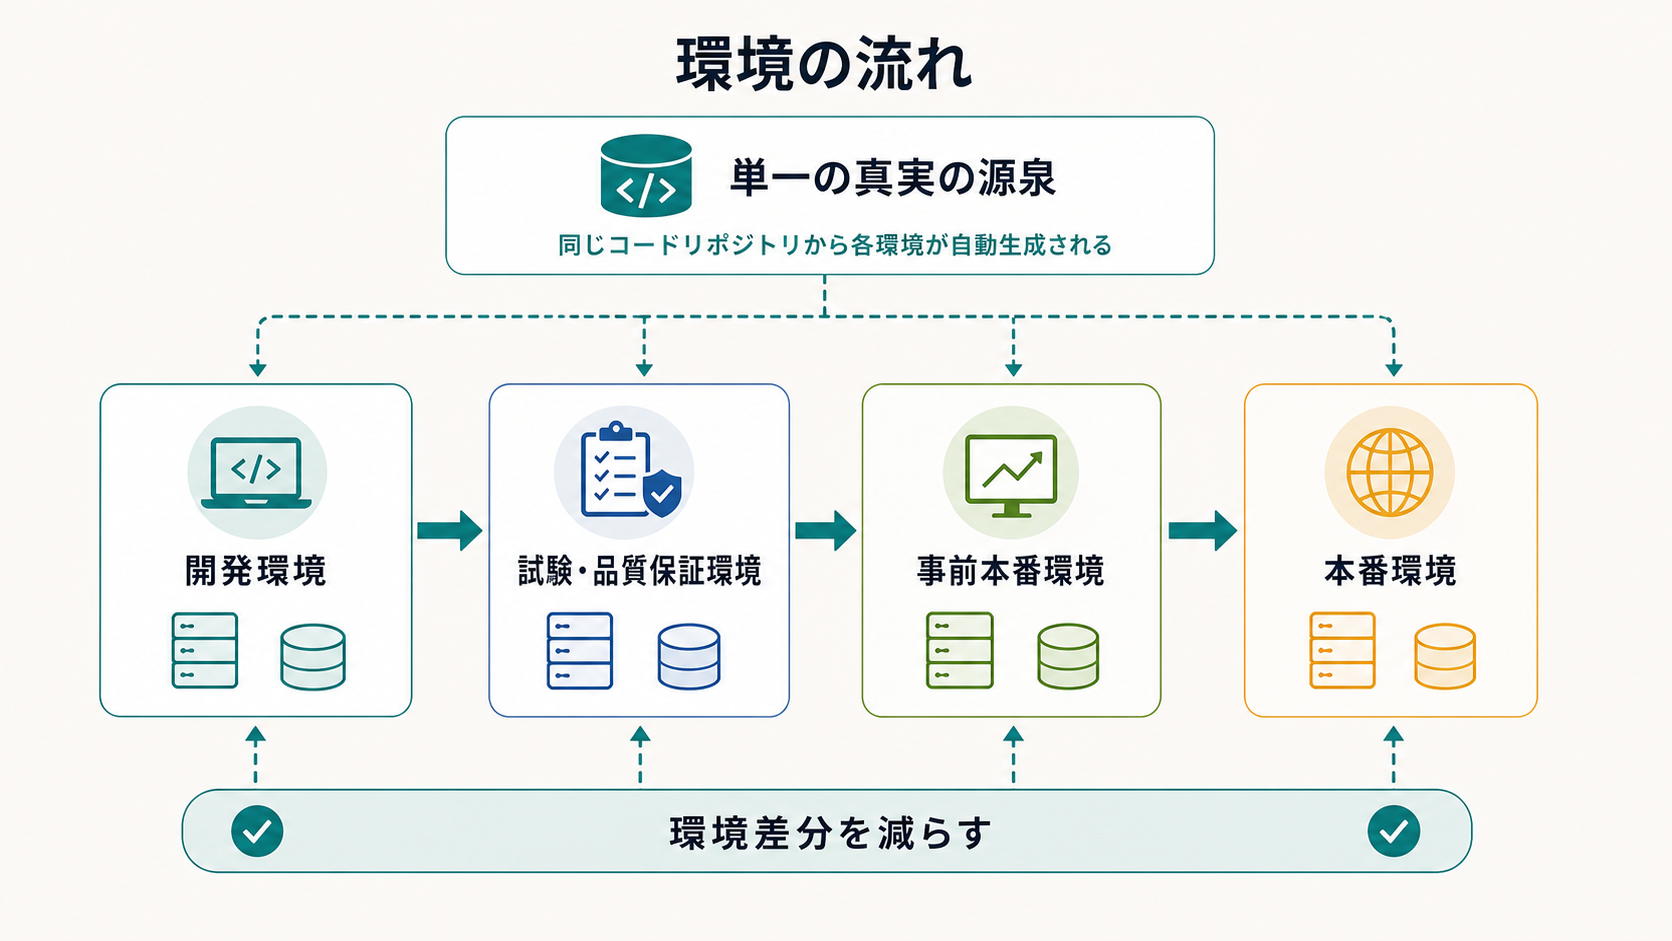
\includegraphics[width=0.96\linewidth]{assets/generated_figures/ch06/fig-ch06-04.png}}{\fbox{\parbox[c][48mm][c]{0.9\linewidth}{\centering 画像生成待ち\\環境の流れ}}}
\caption{環境の流れ}
\label{fig:ch06-04}
\end{figure}

\subsubsection{ソフトウェア可用性、継続性、サービス水準}

可用性とは、必要なときにサービスが利用可能である度合いである。継続性とは、大きな障害や災害が発生してもサービスを維持または復旧できる能力である。サービス水準とは、可用性、性能、応答時間、復旧時間などについて合意された水準である。

運用担当技術者は、プロジェクト初期に非機能要求として定義された可用性と継続性を満たすため、適切なインフラを計画、設計、実装、試験する。可用性は測定され、記録され、予定外の停止は調査される。サービス報告では、合意されたサービス水準に対して、実際の運用がどうだったかを示す。

SLAは、運用サービスの義務を明確にするために有効である。SLAがなければ、利用者は「常に速く、絶対に止まらない」ことを期待し、提供者は「通常は動いている」と考えるかもしれない。合意された水準がなければ、運用の成否を客観的に判断しにくい。

\subsubsection{ソフトウェア容量管理}

容量管理とは、現在と将来の需要に対して、十分な処理能力、記憶容量、ネットワーク、データベース性能などを確保する活動である。利用者数、トランザクション数、データ量、業務量の変化を予測し、それを具体的な要求に変換して文書化する。

容量管理は、性能と容量の問題の中心となる。新規サービスや変更サービスを設計するとき、想定負荷を見積もり、必要な資源をモデル化する。容量計画には、現在の性能、将来要求、費用を伴う選択肢、SLA達成のための推奨策を含める。

\begin{pointbox}{例}
動画配信サービスで、通常時は一日10万人が利用するが、イベント配信時には同時接続が10倍になると予測される場合、容量管理ではピーク時のサーバ数、ネットワーク帯域、キャッシュ戦略、負荷分散、監視しきい値を計画する必要がある。
\end{pointbox}

\subsubsection{バックアップ、災害復旧、フェイルオーバー}

バックアップとは、データ、文書、ソフトウェアを復旧できるように複製して保管することである。災害復旧とは、大規模障害や災害後にサービスを復元する活動である。フェイルオーバーとは、主系が故障したときに、予備系へ切り替えてサービスを継続する仕組みである。

復旧を成功させるには、どのバックアップ方式を使うか、どの頻度で復元点を作るか、どこに保管するか、どれくらい保持するかを決める必要がある。完全バックアップは全体を保存する方式であり、増分バックアップは前回からの差分を保存する方式である。

重要なのは、バックアップを取ることではなく、復旧できることである。災害復旧とフェイルオーバーは、計画され、定期的にリハーサルされる必要がある。ソフトウェア側にも障害処理の論理が必要であり、これは開発時に計画されなければならない。

\begin{figure}[htbp]
\centering
\IfFileExists{assets/generated_figures/ch06/fig-ch06-05.png}{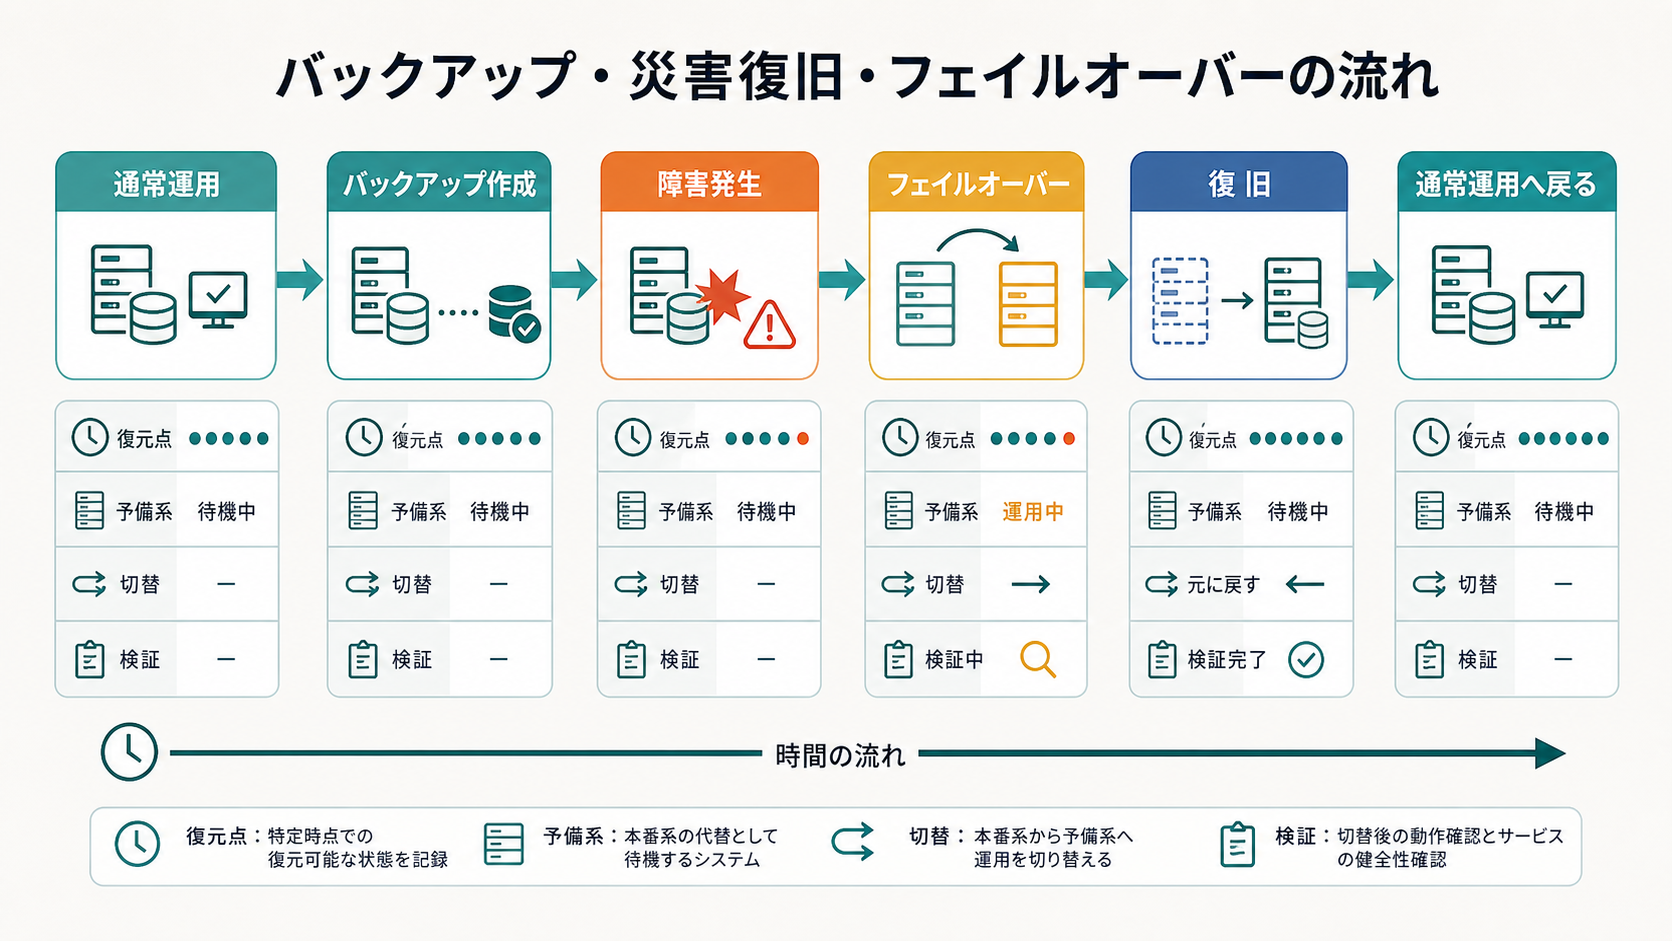
\includegraphics[width=0.96\linewidth]{assets/generated_figures/ch06/fig-ch06-05.png}}{\fbox{\parbox[c][48mm][c]{0.9\linewidth}{\centering 画像生成待ち\\バックアップ・災害復旧・フェイルオーバーの流れ}}}
\caption{バックアップ・災害復旧・フェイルオーバーの流れ}
\label{fig:ch06-05}
\end{figure}

\subsubsection{ソフトウェアとデータの安全性、セキュリティ、完全性、保護、統制}

運用では、情報セキュリティをすべてのサービス活動の中で管理する必要がある。これは、情報の安全性と可用性に関するリスク評価を行い、統制を実施することである。

運用で考えるべき統制には、経営層による情報セキュリティ方針の定義、役割と責任の割当、方針の有効性を監視する責任者、セキュリティ教育、全職員への方針周知、リスク評価と統制実装に関する専門的支援、変更が統制を壊さないことの確認、セキュリティインシデントの報告と対応が含まれる。

DevOpsの発展に伴い、開発運用セキュリティ連携（DevSecOps）が重要になっている。DevSecOpsでは、セキュリティを後工程で追加するのではなく、開発と運用の最初から組み込み、セキュリティ問題の検出と修正をできるだけ早く自動化する。

\begin{figure}[htbp]
\centering
\IfFileExists{assets/generated_figures/ch06/fig-ch06-06.png}{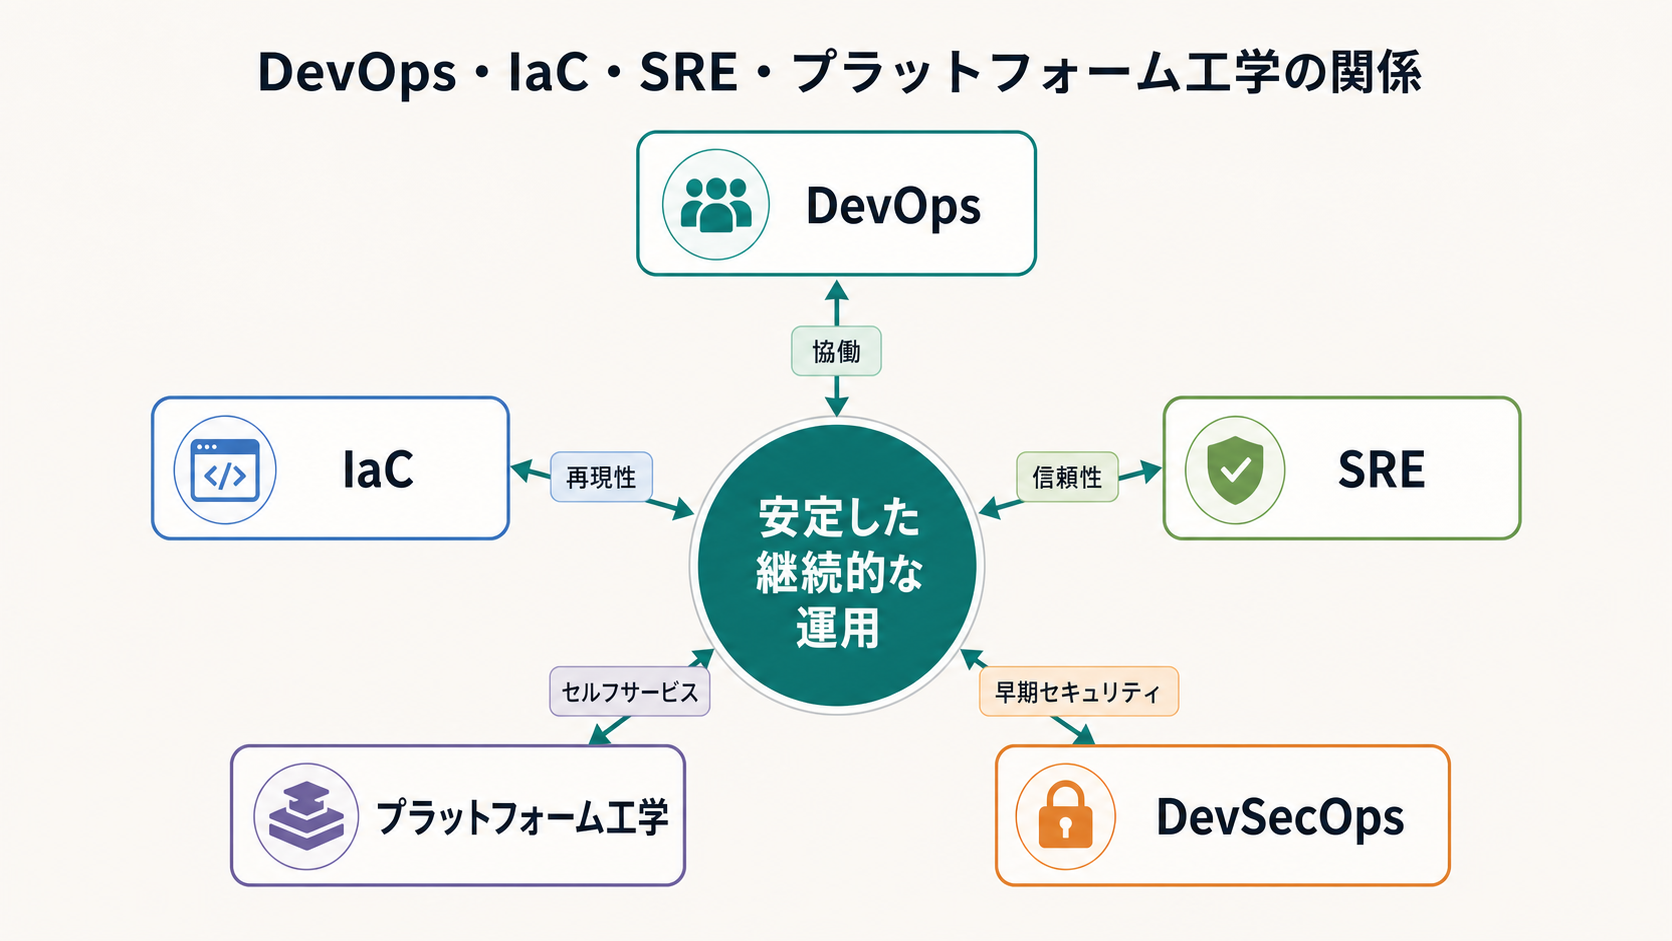
\includegraphics[width=0.96\linewidth]{assets/generated_figures/ch06/fig-ch06-06.png}}{\fbox{\parbox[c][48mm][c]{0.9\linewidth}{\centering 画像生成待ち\\DevOps・IaC・SRE・プラットフォーム工学の関係}}}
\caption{DevOps・IaC・SRE・プラットフォーム工学の関係}
\label{fig:ch06-06}
\end{figure}
